\chapter{Research Method}\label{chp:researchMethod}


%===================================================================================================%
\section{Introduction}
%===================================================================================================%

After exploring the academic body of knowledge in chapter~\vref{chp:background}, 


%===================================================================================================%
\section{Method Evaluation}
%=======================================================%

There are several competing methodological approaches to assess the aptness of technologies in the domain of information systems. In the following section four of these are introduced, discussed and evaluated for further use.

    
    %-------------------------------------%
    \subsection{Task-Technology-Fit}
    %-------------------------------------%
    \begin{figure}[ht]
        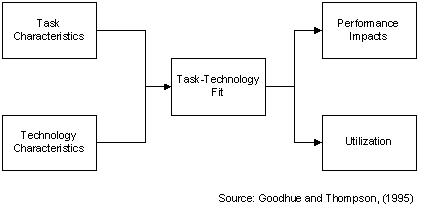
\includegraphics[width=0.7\linewidth]{images/methodology/ttf.jpg}\centering
        \caption
        [Task-Technology-Fit Model]
        {Task-Technology-Fit Model Source: \cite{Goodhue1995Task-TechnologyPerformance}}
    \end{figure}
    
    One of the oldest holistic models for assessing the fit of a given technology is called the "Task-Technology-Fit" (TTF) model. It originates in 1995 and is based on theories of user attitudes, beliefs and behaviors. It implies that a better fit of a technology for a task will result in increased utilization and will have a positive performance impact. Goodhue and Thompson developed a measure that consists of the eight factors:
    \begin{enumerate}[nolistsep]
        \item[\textbf{1}] Quality
        \item[\textbf{2}] Locatability
        \item[\textbf{3}] Authorization
        \item[\textbf{4}] Compatibility
        \item[\textbf{5}] Ease of Use/Training
        \item[\textbf{6}] Production Timeliness
        \item[\textbf{7}] Systems Reliability
        \item[\textbf{8}] Relationship with Users
    \end{enumerate}
    It is apparent that these eight factors are focused on the user of the technology and rely on subjective user-perception. Although Goodhue and Thompson developed their methodology for the individual level of analysis, Zigurs and Buckland refined it for application on group level.\autocite{Zigurs1998AEffectiveness} As mentioned before, this basic TTF model heavily relies on the subjective perception of the user and therefore often operates with surveys or interviews. Since TTF is a very generalistic and holostic approach, it was applied on various domains of information systems and has been combined or used with other related models with great success.\\ 
    However, it is very uncommon to use the TTF in its original, unaltered form but rather modify it to suit the purpose of the particular study since different fields of study require different validation methods. For the technical evaluation of serverless architectures in the context of IoT Event-Stream-Processing the TTF perspective of defining \textit{Task Characteristics} and \textit{Technology Characteristics} to assess the fit and therefore the \textit{Performance Impacts} and \textit{Utilization} but the suggested validation methods (i.e., survey or interview) are not applicable for this study. It is therefore necessary to look at different models and define a research methodology that is fitting for the study at hand. 
    
     %-------------------------------------%
    \subsection{Fit-Viability Model}
    %-------------------------------------%
    \begin{figure}[ht]
        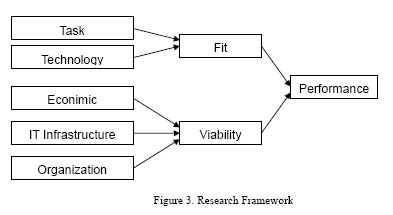
\includegraphics[width=0.7\linewidth]{images/methodology/fvm.jpg}\centering
        \caption
        [Fit-Viability-Model]
        {Fit-Viability-Model Source: \cite{Liang2007AdoptionModel}}
    \end{figure}
    The "Fit-Viability Model" (FVM) for evaluating organizational adoption of technologies was originally proposed by Tjan in 2001 and refined by Liang in 2007. As an extension of the Task-Technology-Fit model it adopts the technology's fit but also introduces the "viability" dimension. Similarly to the approach outline in the last paragraph, FVM assesses the fit be evaluating how well the studied technology fits for the given task in order to gain insights on how well it impacts the performance and utilization. The added dimension of viability is very interesting and important for this study since it includes the economic perspective on the solution and also enables the researcher to focus on the realistic implementation and use of the technology. Similarly to TTF, it is rather vague in recommending specific validation methods and needs to be modified to fit the study. 
    
    %-------------------------------------%
    \subsection{Prototyping}
    %-------------------------------------%
    "Prototyping" refers to the practice of building functioning versions of a system in order to observe its behaviour and derive conclusions on how the productive version would behave.\autocite{Budde1992Prototyping} Since it is a common approach for business and hobbyists alike, a concise and generally accepted definition is hard to find because the understanding can differ vastly depending on the person or organization using it. For research purpose, this paper focuses on the two most important academic sources on the topic: Budde (1992) and Nielsen (1993).\\
    Nielsen defines two different types of prototypes:
    
    \begin{figure}[ht]
        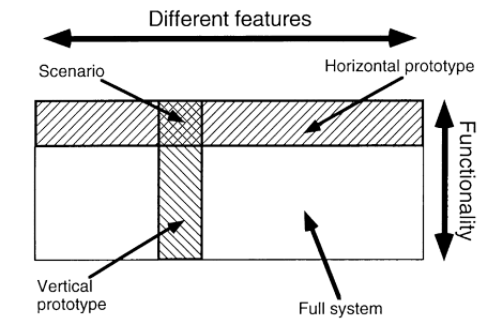
\includegraphics[width=0.7\linewidth]{images/methodology/nielsenProto.PNG}\centering
        \caption
        [The two dimensions of prototyping]
        {The two dimensions of prototyping Source: \cite{Nielsen1993UsabilityEngineering}}
    \end{figure}
    
    \begin{enumerate}
        \item \textbf{Horizontal Prototype}\\
            By reducing the level of functionality, the result of horizontal prototyping is \blockquote{a simulation of the interface where no real work can be performed. [...] This would mean that users should be able to execute all navigation and search commands but without retrieving any real information as a result of these commands}.\autocite{Nielsen1993UsabilityEngineering} The goal is to test the entire user interface without needing to develop the underlying systems. The main advantage of horizontal prototyping is that it provides a rapid feedback-loop between researcher and user by reducing the development time but still delivering a fully functional prototype. In addition, a quick, cost-effective confirmation of the requirements and system scope can be done and first estimates of development time, cost and effort conducted. Moreover, it is an excellent way to showcase the running system to gain a business advantage.\autocite{Nielsen1993UsabilityEngineering}
        \item \textbf{Vertical Prototype}\\
            A vertical prototype is a system that features in-depth functionality but only for a few selected features. Hence, it only provides sufficient test data for a limited part of the system, but it will be tested thoroughly under near real-life conditions. For instance, a vertical prototype of a concert ticket system could feature a fully functional API and processing unit but mocks the database in order to assess only the API and processing unit. 
    \end{enumerate}
    
    Prototyping can be the used to solve various problems and depending on the goal the overall approach can differ vastly. Floyd\autocite{Floyd1984APrototyping} distinguishes between three particular styles of prototyping relating to different goals:
    
    \begin{enumerate}
        \item \textbf{Exploratory Prototyping}\\
            When the problem is unclear, exploratory prototyping is an apt approach for testing initial ideas in order to gain perspective on user and management requirements. Usually, the main focus is to examine a broad variety of design options and to explore these options without premature assumptions or restrictions. As a result, the developer can "play" with various design choices and gain insight into the users' perception of the application. 
        \item \textbf{Experimental Prototyping}\\
            This form of prototyping is closely related to \textit{exploratory prototyping} but focuses on the technical implementation of the development goal. By designing reference systems within the defined problem's scope, the researcher gains insight into suitability and feasibility of a particular application system. The most common approach is to define an experimental environment with disclosed parameters, design several prototypes, determine indices to measure and lastly observe the prototypes' behavior in the experimental environment. Afterwards, the results from each prototype are compared and a technical recommendation is formulated. 
        \item \textbf{Evolutionary Prototyping}\\
            Contrary to the two types mentioned before, with evolutionary prototyping, the prototype is not merely used as a single-use tool in the context of an experiment or research endeavour, but is rather part of a continuous process for adapting a system to various constraints and environment properties. As a result, software development is not seen as a self-contained venture, instead it is organized as a continuous improvement cycle where the prototype is refined in an iterative process until the prototype becomes the final productive release. The aim is to improve the prototype throughout the steps of development in order to eliminate the differences between prototypes and application systems. In comparison to exploratory and experimental prototyping, evolutionary prototyping is therefore very focused on working towards a productive release. The former methods are hence called "throw-away prototyping" approaches.\cfcite{Crinnion1991EvolutionaryMethodology}
    \end{enumerate}
    
    %-------------------------------------%
    \subsection{Requirements Engineering}\label{sssec:reqEng}
    %-------------------------------------%
    "Requirements engineering is the branch of software
    engineering concerned with the real-world goals for,
    functions of, and constraints on software systems. It
    is also concerned with the relationship of these
    factors to precise specifications of software behavior,
    and to their evolution over time and across software
    families."\autocite{Zave1997ClassificationEngineering}
    
    This definition is very appealing for a number of reasons. To begin with, it emphasizes the focus on "real-world goals" that have to addressed in order to create value. These goals define \textit{why} the system should be built and \textit{what} the system's purpose is. In addition, it mentions "precise specification" which provide the the basis for requirements that shape how the software will behave. \textit{Requirements Engineering} is therefore the method of defining and documenting requirements for a software. There is no specific, generally accepted\autocite{Budde1992Prototyping}$^{,}$\autocite{Sommerville1999RequirementsGuide}$^{,}$\autocite{Sommerville2010SoftwareEngineering} toolset of best practices and methods but rather a common understanding what requirements engineering should achieve: 
    \begin{itemize}
        \item Identification of Requirements\\
            Understand the features and functionality the task's environment demands
        \item System Modeling (see \textit{Prototyping})\\
            Design a reference system 
        \item Requirements Specification\\
            Specify the identified requirements further
        \item Requirements Validation\\
            Validate the identified and specified requirements
    \end{itemize}
    
    To validate the identified requirements, a quantitive expert survey will be conducted. A "Likert Scale" \autocite{Likert1932AAttitudes} will be utilized as a proven method to create a standardized questionnaire that presents the respondents all requirements and allows them to rate each requirement. The goal is to objectively evaluate which system properties will be tested in the following sections.
    
    The Likert scale is one if the most frequently used form of attitude measurement in survey research. Like most psychometric scale measures, the Likerts scale employs the approach to list multiple statements that the interviewees can rank corresponding to their level of agreement. An example can be seen at Figure~\vref{fig:likertExample}. Each item uses the same bipolar set of response option expressing agreement or disagreement with the statement (e.g., \textit{Good performance is important for a proper database}. Both ends of the scale are labeled accordingly. \autocite{Brill2008LikertScale}
    
    \begin{figure}[ht]
        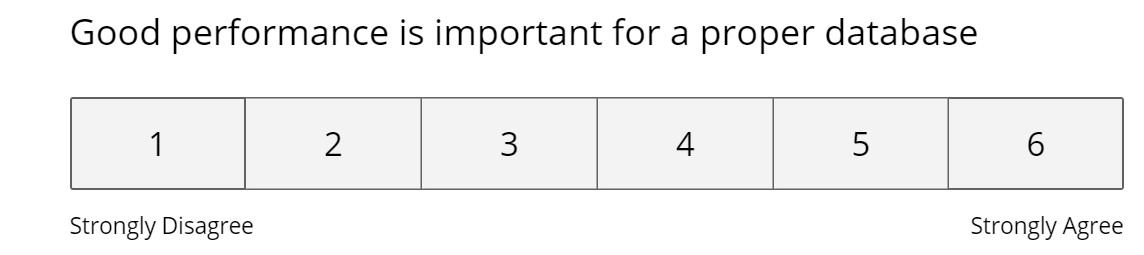
\includegraphics[width=\linewidth]{images/methodology/likert.PNG}\centering
        \caption
        [Likert Scale Example]
        {Likert Scale Example}
        \label{fig:likertExample}
    \end{figure}
    
    

\begin{minipage}{\textwidth}
    %-------------------------------------%
    \section{Conclusion}
    %-------------------------------------%
    
    \subsection{Approach}\label{sec:approach}
    Evaluation of two ESP Data-Consumer Approaches
    \begin{enumerate}
        \item \textbf{Requirements Engieering}\\
            Based on Suitability (TTF) \& Viability (FVM)
            \begin{enumerate}
                \item[I.] \textbf{Requirements Identification} (LiteratureReview)\\
                    $\longrightarrow$ \textbf{Requirements Specification}(Hypothesis)
                \item[II.] \textbf{Requirements Validation/Selection}(Quantitative Survey, Likert Scale)
            \end{enumerate}
        \item \textbf{Environment/Task Modelling}
        \item \textbf{Prototype Modelling}
        \item \textbf{Evaluation of Prototypes} (Based on Requirements)
        \item \textbf{Recommendation}
    \end{enumerate}
    
    After evaluating different methods and their characteristics, an approach combined out of components from the Task-Technology-Fit Model and Fit-Viability Model is chosen to define environment attributes and conditions. Using literature research combined with requirement engineering, indices and variables to be measured will be determined. Requirements that are identified via this approach will be validated through a quantitative survey. The suitability and viability of the examined prototypes will be decisive for the architectural recommendation and will result in an answer to the research question and objective.\\
    Since this study aims to answer the question whether and under which circumstances serverless architectures are a good fit for IoT Event-Stream-Processing, an experimental, vertical prototype is best suited as a method of validation. 
    
\end{minipage}



%===================================================================================================%
\section{Summary}\label{chp:researchMethodEND}
%===================================================================================================%

\begin{enumerate}[nolistsep]
        \item \textbf{Requirements Engieering}\\
            Based on Suitability (TTF) \& Viability (FVM)
            \begin{enumerate}
                \item[I.] \textbf{Requirements Identification} (LiteratureReview)\\
                    $\longrightarrow$ \textbf{Requirements Specification}(Hypothesis)
                \item[II.] \textbf{Requirements Validation/Selection}(Quantitative Survey, Likert Scale)
            \end{enumerate}
        \item \textbf{Environment/Task Modelling}
        \item \textbf{Prototyping}
        \item \textbf{Suitability Assessment} 
        \item \textbf{Viability Assessment}
        \item \textbf{Recommendation $\longrightarrow$ Conclusion}
\end{enumerate}

After evaluating different methods and their characteristics, an approach combined out of components from the Task-Technology-Fit Model and Fit-Viability Model is chosen to define environment attributes and conditions. Using literature research combined with requirement engineering, indices and variables to be measured will be determined. Requirements that are identified via this approach will be validated through a quantitative survey. 

As a methodological approach for the quantitive survey, a Likert scale was employed since the study benefits from its academic advantages and the impact of its response distortions if minimal. The bipolar response option set \textit{Not Important} and \textit{Very Important} was used to let the respondents (technical experts in the field of IoT, Event-Stream-Processing and Serverless) express their personal prioritization of various system properties. To emphasize the equidistance between the options, a consecutive set of integers (ranging from 1 to 6) was employed as scale labels. The Likert items are as follows:

\begin{enumerate}[nolistsep]
    \item \textbf{Ease of Development}\\
        Including: Quality/Comprehensiveness of Documentation, Available Tooling, Ease of Testing (Unit, Integration, User Acceptance, etc.), Debugging, ...
    \item \textbf{Ease of Operation}\\
        Including: Monitoring, Deployment, Versioning, Performance Optimization, ...
    \item \textbf{Feature Velocity}
    \item \textbf{Low Vendor Lock-In}
    \item \textbf{Cost}\\
        Including: Overall Cost of Operation/Ownership, Cost-Control, Ease of Billing/Payment, Total Costs of Maintenance, ...
    \item \textbf{Automated/Limitless Scaling}
    \item \textbf{Event-Driven Design}
    \item \textbf{Low Latency}\\
         Message Received - Message Processed
    \item \textbf{Failure Resilience}\\
         Automatic Failover Strategies, Outage Mitigation, Self-Healing Capabilities
    \item \textbf{Message Throughput}
\end{enumerate}

After calculating the average response value for each item, the two items with the highest value in the categories \textit{suitability} and \textit{viability} will be chosen to be examined in the next steps.\\
A testing environment and task will be constructed based on the two chosen system properties from the previous step. 
The suitability and viability of the examined prototypes will be decisive for the architectural recommendation and will result in an answer to the research question and objective.
Since this study aims to answer the question whether and under which circumstances serverless architectures are a good fit for IoT Event-Stream-Processing, an experimental, vertical prototype is best suited as a method of validation. 